\tikzsetfigurename{module6_9_localeOptima}
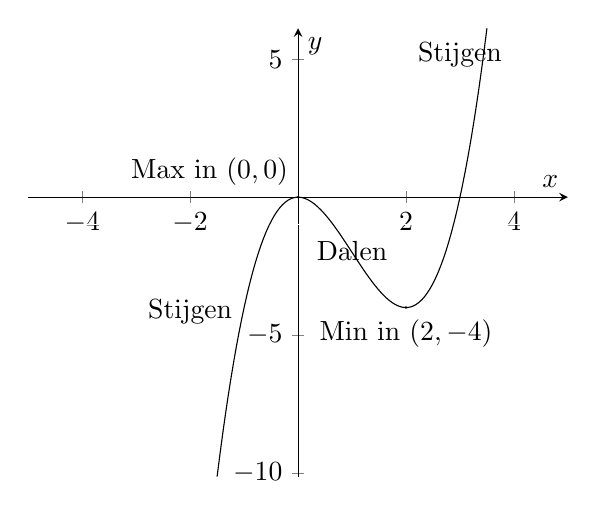
\begin{tikzpicture}

\begin{axis}[xlabel=$x$,
ylabel=$y$,
axis lines = middle]

\addplot[mark=none,color=white] {-1};
\addplot[mark=none, domain=-1.5:3.5, samples=100,color=black] {x^3-3*x^2};

\node[label={100:{Max in $(0,0)$}},circle,fill,inner sep=0.1pt] at (axis cs:0,0) {};
\node[label={270:{Min in $(2,-4)$}},circle,fill,inner sep=0.1pt] at (axis cs:2,-4) {};
\node[label={270:{Stijgen}}] at (axis cs:-2,-3) {};
\node[label={90:{Dalen}}] at (axis cs:1,-3) {};
\node[label={90:{Stijgen}}] at (axis cs:3,4) {};

\end{axis}


\end{tikzpicture}